\section{What changed between the two releases?}

\begin{table}[!b]
\centering
\caption{Primary 64-country contrasts. $\Delta$ is GPT-5.6 Sol minus GPT-5.5 target loss; negative values favor GPT-5.6. Intervals resample countries and Holm correction spans five global metrics.}
\label{tab:main}
\small
\setlength{\tabcolsep}{4.2pt}
\begin{tabular*}{\linewidth}{@{\extracolsep{\fill}}lrrrl@{}}
\toprule
\rowcolor{tablehead}
Metric target & $\Delta$ loss & 95\% BCa CI & Holm $p$ & Corrected read \\
\midrule
W1 $\downarrow$ & -0.0020 & [-0.0040,0.0003] & 0.319 & uncertain \\
\rowcolor{improvebg}
TVD $\downarrow$ & \textbf{-0.0080} & \textbf{[-0.0107,-0.0050]} & \textbf{$<0.001$} & \textbf{lower error} \\
CRG $\downarrow$ & -0.0022 & [-0.0243,0.0215] & 0.845 & uncertain \\
VDR $\to 1$ & -0.0220 & [-0.0506,0.0025] & 0.319 & uncertain \\
CSR $\uparrow$ & 0.0333 & [-0.0082,0.0834] & 0.319 & uncertain \\
\bottomrule
\end{tabular*}
\vspace{1pt}\parbox{.98\linewidth}{\small W1 measures ordered displacement; TVD measures category mass; CRG measures profile error. VDR and CSR target cross-country spread and relational ordering. Model levels and standard errors appear in Appendix Table~\ref{tab:global-estimates}.}
\end{table}


Table~\ref{tab:main} gives the five global comparisons. Only the six-item
total-variation distance (TVD) improves after correction:
$\Delta=-0.0080$ (95\% BCa CI $[-0.0107,-0.0050]$, Holm $p<0.001$).
W1, CRG, and the target-loss contrasts for VDR and CSR remain inconclusive.
Reduced category-mass error does not establish improved ordering or geometry.

The corrected 12-outcome item family finds Q108 responsibility improved under
W1 and TVD and Q106 income distribution improved under TVD; no other item passes
joint correction. These two items contribute 98.0\% of the signed six-item TVD
point reduction. In exploratory omissions, TVD remains negative after excluding
Q106 ($-0.00433$, CI $[-0.00698,-0.00138]$), but removing both Q106 and Q108
leaves a near-zero contrast ($-0.00024$, CI $[-0.00313,0.00286]$). The Q106
item-specific gain cannot be verified with corrected wording from these outputs;
Appendix~\ref{app:results} reports all exclusions and the Q121 bounds.

The five-run mean removes 1.18\% of GPT-5.5 and 1.31\% of GPT-5.6 single-run
squared probability error (Figure~\ref{fig:results}b). The GPT-5.6 residual
falls by $0.0063$ (95\% CI $[-0.0083,-0.0045]$), whereas run-varying error
does not reliably differ. Spatial-error and spatial-HAC intervals for the
global TVD contrast remain below zero over the tested graphs and cutoffs.
These checks support a mean contrast on the derivative, without measuring
diffusion or causal effects.

\begin{figure}[t]
  \centering
  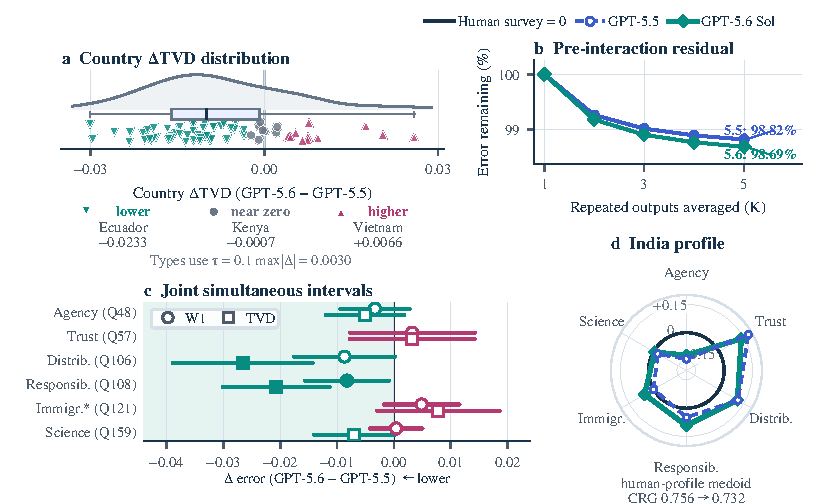
\includegraphics[width=\linewidth]{figs/fig2_multiview_results.pdf}
  \caption{Four views of the update. \textbf{a}, country TVD changes and threshold-defined
  examples. \textbf{b}, exact error remaining after averaging subsets of five outputs.
  \textbf{c}, simultaneous 95\% W1/TVD intervals; circles denote W1, squares TVD, and
  fill max-$T$ significance. \textbf{d}, India's model-minus-survey profile on a common
  $[-0.20,+0.20]$ scale; the outcome-free human-profile medoid has CRG
  $0.756\rightarrow0.732$. The zero ring is the survey baseline, not a normative target.
  Appendix Figure~\ref{fig:country-profiles-appendix} shows the three CRG-class medoids.}
  \label{fig:results}
\end{figure}
